\section*{CHƯƠNG 2. TẬP DỮ LIỆU VÀ TIỀN XỬ LÝ}
\setcounter{section}{2}
\setcounter{subsection}{0}
\addcontentsline{toc}{section}{Chương 2. Tập dữ liệu và Tiền xử lý}

\subsection{Mô tả bộ dữ liệu chuẩn MNIST}
Bộ dữ liệu MNIST bao gồm $70.000$ mẫu ảnh chữ số viết tay từ $0$ đến $9$. Mỗi bức ảnh có kích thước cố định $28 \times 28$ pixel mức xám (grayscale), được căn giữa và chuẩn hóa kích thước nét vẽ.

Dữ liệu được phân chia theo tỷ lệ chuẩn mực và cố định seed ngẫu nhiên ($42$) lưu trong \code{split\_indices.npz}:
\begin{itemize}
    \item \textbf{Tập huấn luyện (Training Set):} $50.000$ mẫu ảnh, dùng để tối ưu hóa tham số nội tại ($W, b$ hoặc bảng xác suất $\theta$).
    \item \textbf{Tập kiểm định (Validation Set):} $10.000$ mẫu ảnh, dùng để tinh chỉnh siêu tham số và kích hoạt cơ chế Dừng sớm.
    \item \textbf{Tập kiểm thử độc lập (Test Set):} $10.000$ mẫu ảnh, hoàn toàn độc lập dùng để đánh giá năng lực khái quát hóa cuối cùng.
\end{itemize}

\begin{figure}[htbp]
    \centering
    \begin{subfigure}[b]{0.48\textwidth}
        \centering
        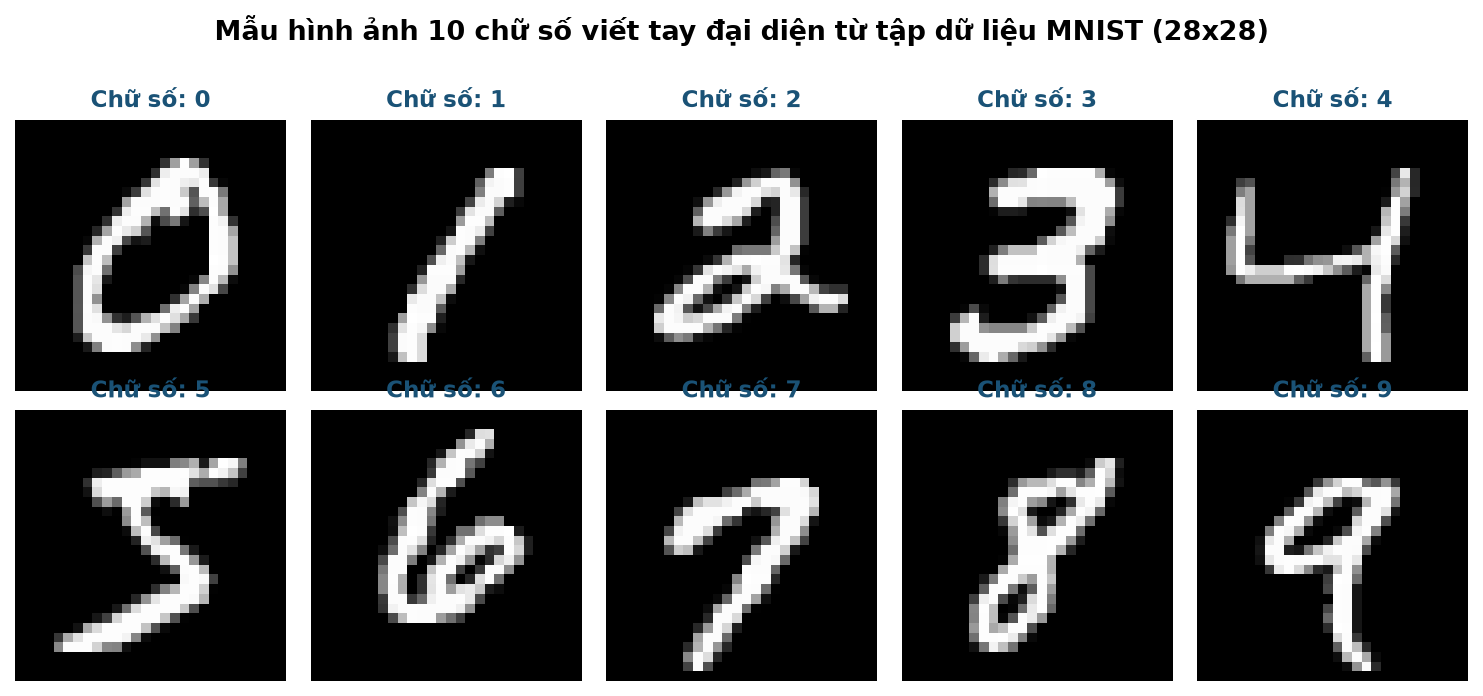
\includegraphics[height=3.3cm, keepaspectratio]{figures/0_01_sample_digits.png}
        \caption{Mẫu ảnh ngẫu nhiên từ 10 lớp chữ số}
        \label{fig:0_01_samples}
    \end{subfigure}
    \hfill
    \begin{subfigure}[b]{0.48\textwidth}
        \centering
        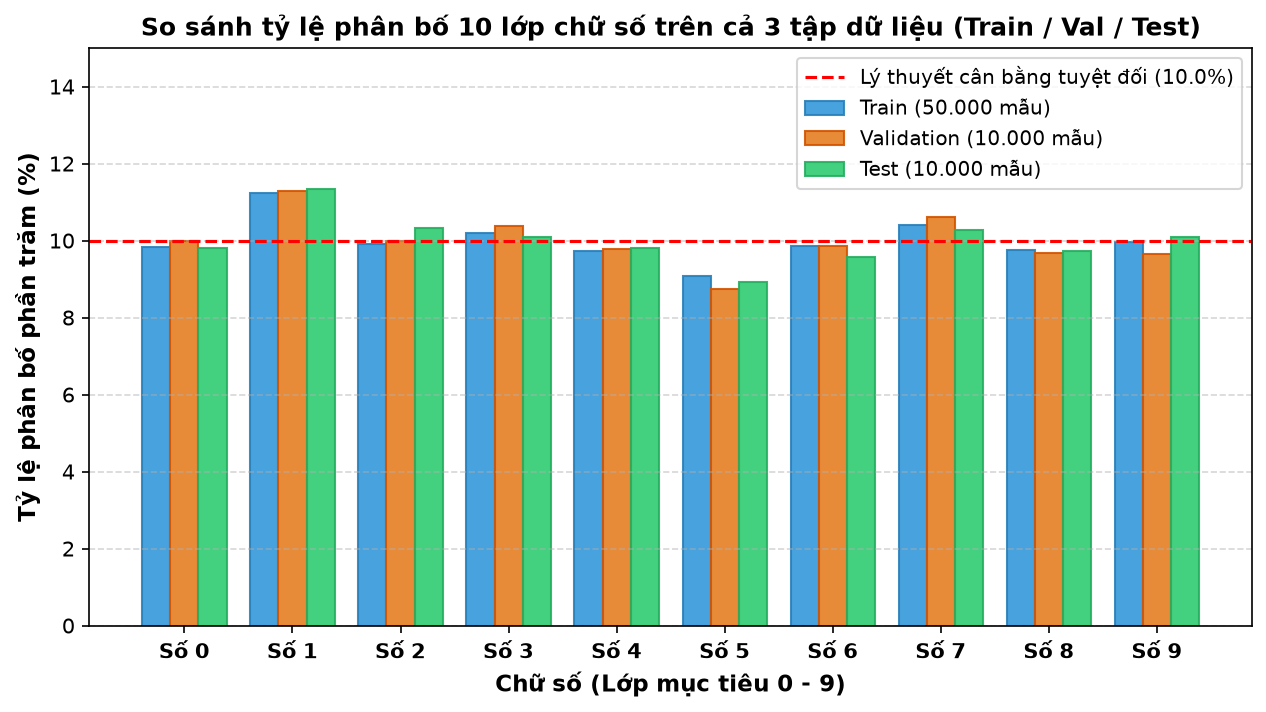
\includegraphics[height=3.3cm, keepaspectratio]{figures/0_02_class_distribution.png}
        \caption{Phân phối số lượng mẫu giữa các tập}
        \label{fig:0_02_dist}
    \end{subfigure}
    \caption{Khảo sát trực quan tập dữ liệu MNIST}
    \label{fig:dataset_overview}
\end{figure}

Như thể hiện trên Hình~\ref{fig:0_02_dist}, tỷ lệ các lớp chữ số trong cả ba tập phân chia đều xấp xỉ $10\%$ mỗi lớp (dao động từ $9.5\%$ đến $10.5\%$). Sự cân bằng lớp này giúp việc đánh giá bằng các chỉ số như Accuracy và Macro-F1 phản ánh trung thực và đồng nhất năng lực của các mô hình.

\subsection{Phân tích khám phá hình thái học (EDA)}
Chúng ta tính toán vector kỳ vọng $\boldsymbol{\mu}_c \in \mathbb{R}^{784}$ và vector phương sai $\boldsymbol{\sigma}_c^2 \in \mathbb{R}^{784}$ cho từng lớp chữ số $c \in \{0, \dots, 9\}$:
\begin{equation}
    \boldsymbol{\mu}_c = \frac{1}{N_c} \sum_{j: y^{(j)}=c} \mathbf{x}^{(j)}, \qquad \boldsymbol{\sigma}_c^2 = \frac{1}{N_c} \sum_{j: y^{(j)}=c} (\mathbf{x}^{(j)} - \boldsymbol{\mu}_c)^2
\end{equation}

\begin{figure}[htbp]
    \centering
    \begin{subfigure}[b]{0.48\textwidth}
        \centering
        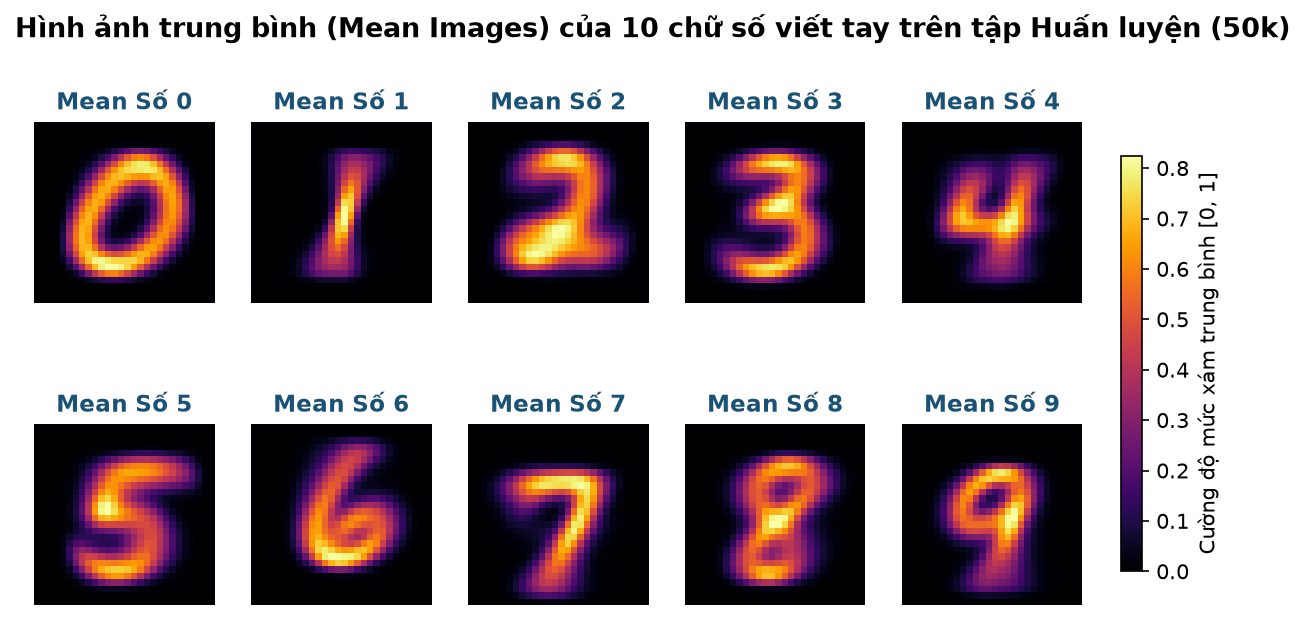
\includegraphics[height=3.3cm, keepaspectratio]{figures/0_03_mean_digits.png}
        \caption{Ảnh trung bình (Mean Digits) của 10 lớp}
        \label{fig:0_03_mean}
    \end{subfigure}
    \hfill
    \begin{subfigure}[b]{0.48\textwidth}
        \centering
        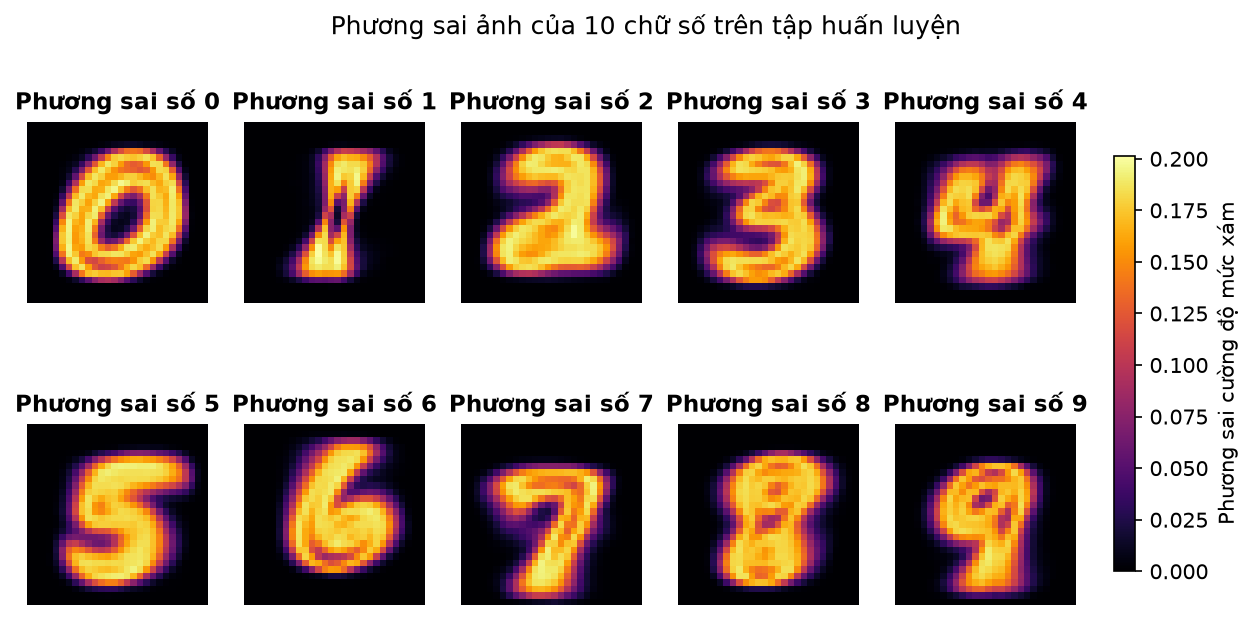
\includegraphics[height=3.3cm, keepaspectratio]{figures/0_04_variance_digits.png}
        \caption{Bản đồ phương sai (Variance Digits) của 10 lớp}
        \label{fig:0_04_var}
    \end{subfigure}
    \caption{Phân tích thống kê điểm ảnh trên từng lớp chữ số MNIST}
    \label{fig:mean_var_analysis}
\end{figure}

Từ Hình~\ref{fig:mean_var_analysis}, ta rút ra hai nhận xét kỹ thuật then chốt:
\begin{enumerate}
    \item \textbf{Vùng biên ảnh hoàn toàn bất hoạt:} Tất cả các điểm ảnh nằm sát mép ngoài ($3-4$ pixel cách biên) đều có giá trị trung bình xấp xỉ $0$ và phương sai xấp xỉ $0$. Thông tin phân loại tập trung trọn vẹn ở vùng trung tâm $20 \times 20$ pixel.
    \item \textbf{Độ biến thiên cao ở các nét uốn và độ nghiêng:} Bản đồ phương sai (Hình~\ref{fig:0_04_var}) cho thấy các vị trí có độ biến thiên cao nhất nằm ở nét gạch ngang của số 4, vòng cung đỉnh của số 8, nét uốn cong của số 2 và góc nghiêng của số 1.
\end{enumerate}

\subsection{Quy trình chuẩn hóa dữ liệu cho từng nhóm thuật toán}
Để phục vụ tối ưu cho từng kiến trúc mô hình, dữ liệu thô được chuẩn hóa và tái định hình:
\begin{itemize}
    \item \textbf{Chuẩn hóa cường độ điểm ảnh:} Toàn bộ giá trị pixel gốc nguyên $x_{ij} \in [0, 255]$ được chia cho $255.0$ để đưa về đoạn số thực $[0.0, 1.0]$. Thao tác này giúp gradient đối xứng, tránh bùng nổ trọng số khi tính tích vô hướng.
    \item \textbf{Định dạng vector $1\text{D}$ cho Naïve Bayes, Logistic, MLP và AdaBoost:} Ma trận ảnh $28 \times 28$ được duỗi phẳng thành vector $\mathbf{x} \in \mathbb{R}^{784}$. Với Naïve Bayes đa thức, việc giữ nguyên miền giá trị không âm $[0, 1]$ tương thích tự nhiên với ước lượng tần suất xuất hiện nét vẽ.
    \item \textbf{Định dạng tensor $4\text{D}$ cho CNN:} Dữ liệu được tái định hình thành tensor kích thước $(N, C, H, W) = (N, 1, 28, 28)$, trong đó $C = 1$ là số kênh mức xám, $H = W = 28$ là kích thước không gian để bộ lọc tích chập khai thác trực tiếp tính liên kết hình học 2D.
\end{itemize}
Dữ liệu tiền xử lý được xuất ra tệp \code{data/processed/mnist\_processed.npz} để đảm bảo tính nhất quán giữa các mô hình.
